\documentclass[titlepage,12pt,twoside,a4paper]{article}

% packages
\usepackage[0.8]{geometry} % set margins
\usepackage{listings}
\usepackage{textcomp}
\usepackage{graphicx}      % for inserting images
\graphicspath{{images/}}     % define the images directory
% turn on page numbers and section name on each page
\pagestyle{headings}

% for multi columns pages
\usepackage{multicol}

% define the formatting for inline code snippets
\newcommand{\code}[1]{{\texttt{#1}}}

% no paragraph indentation
\setlength{\parindent}{0em}

% one line between each paragraph
\setlength{\parskip}{1em}

% Title Page
\title{MIPS PIPELINED PROCESSOR}
\author{
	Abdelrahman Mohamed Abdelnabi\\
	3466
	\and
	Ahmed Atia Lotfey Siam \\
	4129
	\and
	Ahmed Fayez \\
	4130
}

%=====================================%
% DOCUMENT
%=====================================%
\begin{document}
\maketitle

\begin{abstract}
	Pipelining is a powerful way to improve the	throughput of a digital system. We design a pipelined processor by subdividing the single-cycle processor into five pipeline stages. Thus, five instructions can execute simultaneously, one in each stage. Because each stage has only one-fifth of the entire logic, the clock frequency is almost five times faster. Hence, the latency of each instruction is ideally unchanged, but the throughput is ideally five times better. Microprocessors execute millions or billions of instructions per second, so throughput is more important than latency. Pipelining introduces some overhead, so the throughput will not be quite as high as we might ideally desire, but pipelining nevertheless gives such great advantage for so little cost that all modern high-performance microprocessors are pipelined.
	In this Lab, we will design and implement a MIPS piplined  processor using\textit{ System Verilog}.
\end{abstract}

%=====================================%
% CHAPTER 1
%=====================================%


\section{Introduction}
\subsection{Supported Instructions}
\begin{tabular}{ccc}
	\label{ISA}
	% TODO: add table of supported instructions here
	Opcodes & Example Assembly & Semantics \\
	
\end{tabular}

\subsection{Initial Version}
We will use the MIPS pipelined version developed in our textbook as the initial version which we will build on it other components to support the remaining instructions.

This version already supports the instructions:add (\code{add}), sub (\code{sub}), add immediate (\code{addi}), and (\code{and}), or (\code{or}), load word (\code{lw}), sw (\code{sw}), branch on equal (\code{beq}), set on less than (\code{slt}), jump (\code{j}), with a hazard and control unit.

The initial version also uses early branch resolution to make a branch decision in the decode stage.

\subsection{fixing a small error}

The version in the textbook uses an equal comparator in the decode stage for early branch resolution. The datapath module instantiates an \code{eqcmp} object which is not defined in any file. we implemented the module ourselves. You can find the source code of the module in appendix \ref{appendix:src:mipsparts}

The pipelined processor writes the register file in the first half of the write-back stage and reads it the second half of the decode stage. However, this was not the case in the text book code. The register file was written and read at the same time. To fix this, we added a delay of 5 time units after the write.

After this two fixes the test bench indicates a successful simulation.
%=====================================%
% CHAPTER 2
%=====================================%

\section{Extending the Design}

In this section we will modify and/or extend the design of the MIPS pipelined processor to support new instructions as indicated in table \ref{ISA}

\subsection{Branch on Not Equal}
supporting this instruction is relatively easy, as branch on not equal is already supported. We just have to detect the not equal condition. To do this, we modify the control unit to detect the opcode of \code{bne} and generate the required control signals.

We add a new control signal, \code{bneD} which is 1 when the instruction in the decode stage is a \code{bne}. all the control signals for \code{beq} and \code{bne} are same except for the signals \code{branchD} and \code{bneD}, their values are reversed. 

The logic for \code{pcsrcD} is now different. \code{prcsrcD} is now 1 when either of the conditions of \code{beq} and \code{bne} are satisfied. i.e \code{pcsrcD = (branchD \& equalD) | (bneD \& $\sim$equalD)}


The logic for stalling will need to detect the \code{bne} instruction and stall as necessary exactly the same like for \code{beq}. Therefore the hazard unit takes a new input which the control signal \code{bneD}.

This completes all the necessary changes required for the control unit and datapath.

We test the instruction by adding a \code{bne \$s2, \$2, 0x30} after the first instruction of our test program. Testing shows that the stall and branching works properly both when the branch is taken and not taken.

To see the changes to the source code to support this instruction run:\\
\code{git diff abdc c7c0}

\subsection{load byte}

An example of this instruction is \code{lb \$s1, 40(\$s0)}, which loads the byte at the address of 40 + reg(\$s0), sign-extends it and puts it in register \$s1.

To support this instruction we need to select a byte out of the 4 bytes read from memory each cycle according to $memaddr_{[1:0]}$, and then sign extend it to 32 bits. We will need a control signal that tells us that this is a \code{lb} instruction, then at the memory stage, we will select either the 32 bits memory output or the sign extended byte according to this signal. This implies using a 2-1 multiplexer that has this control signal as its selector. We will need another multiplexer to select the proper byte from the memory word read.

We test the instruction by modifying our test program to use \code{lb} instead of \code{lw} (temporarily). Since this should still the load 7 into register \$s2, it won't modify the final result. We run the simulation and it indicates successful completion. we also see that the \code{lbW} signal takes the value 1 only at the write-back stage of the load byte instruction.

To see the changes made to the code to support this instruction run:\\
\code{git diff 18dc 5547}

\subsection{Logical Shift}

logical shift left, \code{sll} and right \code{srl} are R-Type instructions. The infrastructure for R-Type instructions already exists and therefore no significant changes to the datapath are required. Most of the change occurs because of the \textit{shamt} field needs to be passed to the execute stage and the ALU. We add the shamt to the execute stage pipeline register, and modify the ALU to accept it as an input. The ALU decoder will need to detect the shift instructions and generate the proper ALUcontrol signals, so we add 2 rows to the decoder's truth table, one for each instruction. Moreover we extend the ALUControl signal to 4 bits to be able to encode the two new instructions. Table \ref{table:aluctrl} shows new the ALU control signals truth table.

To test the two new instructions, we add \code{sll \$s2, \$s2, 4} and \code{srl \$s2, \$s2, 4} just before the last instruction in out test program. This won't modify the final result since \$s2 contains 7 before running the shift instructions and we shift left then right by the same amount. Running the simulation, the correct result is written and completes successfully.

To see the changes made to the code to support these instructions run:\\
\code{git diff 2656 5ab4} 
\begin{table}
\begin{center}
	
	\begin{tabular}{|c|c|}
		\hline
		$ALUControl_{3:0}$ & Function \\
		\hline
		0000 & A AND B \\
		0001 & A OR B \\
		0010 & A + B \\
		0011 & not used \\
		1000 & A AND $\overline{B}$ \\
		1001 & A OR $\overline{B}$ \\
		1010 & A - B \\
		1011 & SLT \\
		0100 & B \textlangle{}\textlangle{ }shamt \\
		0101 & B \textrangle{}\textrangle{ }shamt \\
		\hline
	\end{tabular}
\end{center}
	\label{table:aluctrl}
	\caption{ALU control truth table}
\end{table}


\subsection{Jump and Link}
The semantics of \code{jal label} is \code{\$ra = PC + 4, goto label}. \code{jal} does exactly the same as jump but writes the value of PC onto register 31, the return address register.

Implementing this instruction won't affect the hardware as much because \code{jal} is mixture of jump and R-Type, both of which are already supported. We will add to the datapath a new mux that selects which data to write to the register file. The new mux will choose between \textit{ResultW} and \textit{PCPlus4W}, according to the selector \textit{jal}, which is a new control signal that is true only if the instruction is \code{jal}. The \textit{PCPlus4} signal must be passed from the decode to the write back stage so that we can write it to the register file. We will also extend the \textit{RegDst} mux, which selects which register to write on, to accept the number 31 as a new input. This means that we need to extend the mux selector control signal, \textit{RegDst}, to 2 bits.

To test the instruction, we modify the test program to use \code{jal} instead of \code{j} on the instruction at address 3C. This won't change the results. It will only write the value of PC + 4, which is 40 at the time of executing the instruction, to the return address register, \$ra.

Figure \ref{jaltest} shows the simulation of the test program with \code{jal} being used. Notice the simulation ends successfully the \textit{jalD} and \textit{jalW} signals are 1 when the instruction is decoded and when the result is written to the register file. Also notice that the return address register has the correct value (0x40) written to it, at the second half of the write back stage of the \code{jal} instruction.

To see the changes made to the code to support this instruction run: \\
\code{}
\begin{figure}
	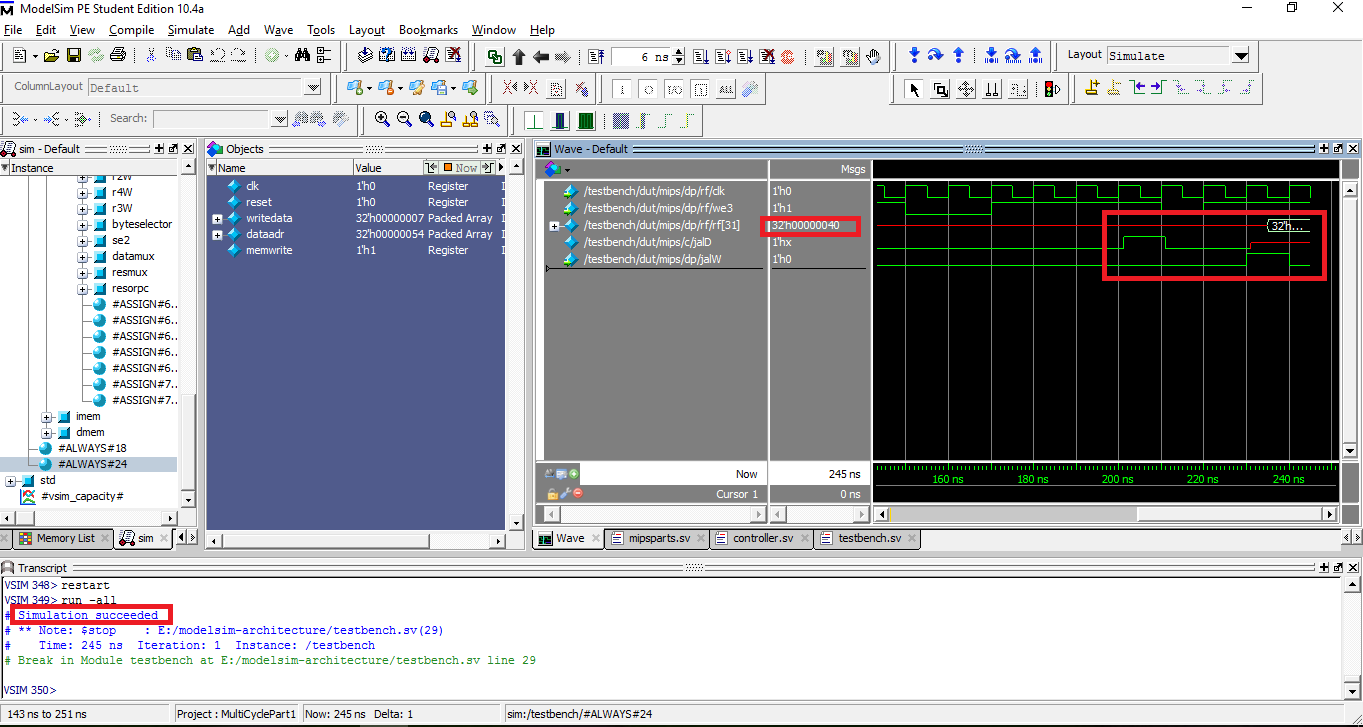
\includegraphics[width=\textwidth]{jaltest.png}
	\centering
	\label{jaltest}
	\caption{simulation and testing of \code{jal}}
\end{figure}

%=====================================%
% Source Code appendix
%=====================================%

\newpage
\appendix
\begin{multicols}{2}
[	
\section{Source Code}
\label{appendix:src}
]
\subsection{maindecoder.sv}
\lstinputlisting[breaklines=true,basicstyle=\tiny,language=verilog]{../maindecoder.sv}

\subsection{mipsparts.sv}
\label{appendix:src:mipsparts}
\lstinputlisting[breaklines=true,basicstyle=\tiny,language=verilog]{../mipsparts.sv}
\end{multicols}
\end{document}          
